\chapter{The PAI Interface}
\label{pai}

The Protolib Application Interface (PAI) provides a layer that allows Protolib to be used Java applications. Specifically, it provides a generic interface to timers, sockets and dispatchers and then employs the use of the \emph{factory method design pattern} in order to instantiate the required set of objects e.g. UDP sockets, TCP NS2 sockets, realtime timers, NS2 timers, NS2 event dispatchers etc.  

The resulting PAI interface looks very similar to a Java interface. Where ever 
possibly, we have used the Java conventions for interfacing with the underlying objects. For example, instead of providing callback functions for a timer, we allow a user to attach multiple listeners to a timer in order to get notified when an event occurs.  The resulting interface therefore is very simple and very Java friendly.  

In this chapter, we give a brief overview of PAI and provide some programming examples of its use. We then show how PAI can be used within NS2 by providing a PAI NS2 agent for integrating with Protolib.

\section{Overview of PAI}

\begin{figure}
\centering
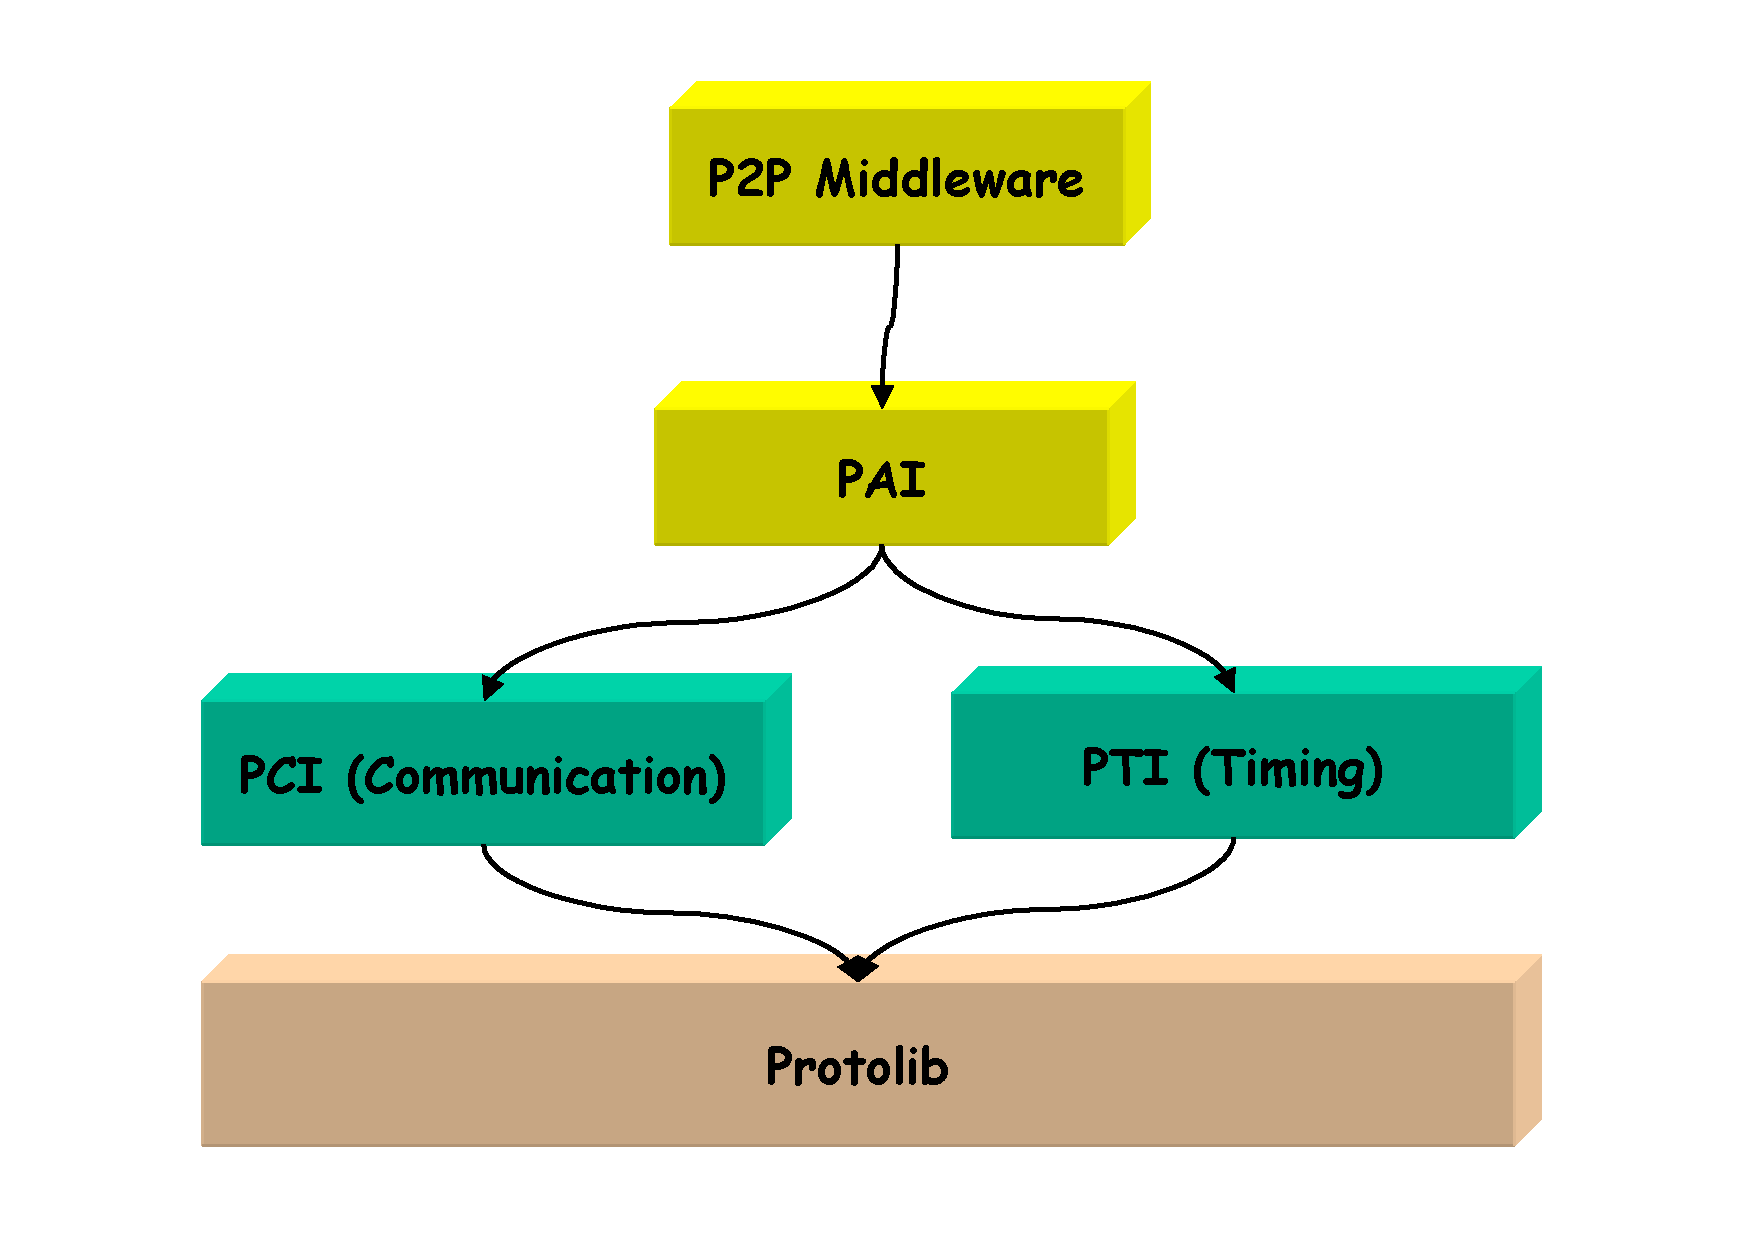
\includegraphics[scale=0.4]{images/paiOverview}
\caption{An overview of the PAI interface, showing the two sections to the
underlying Protolib sockets and timers.} 
\label{pai:fig:overview}
\end{figure}

\begin{figure}
\centering
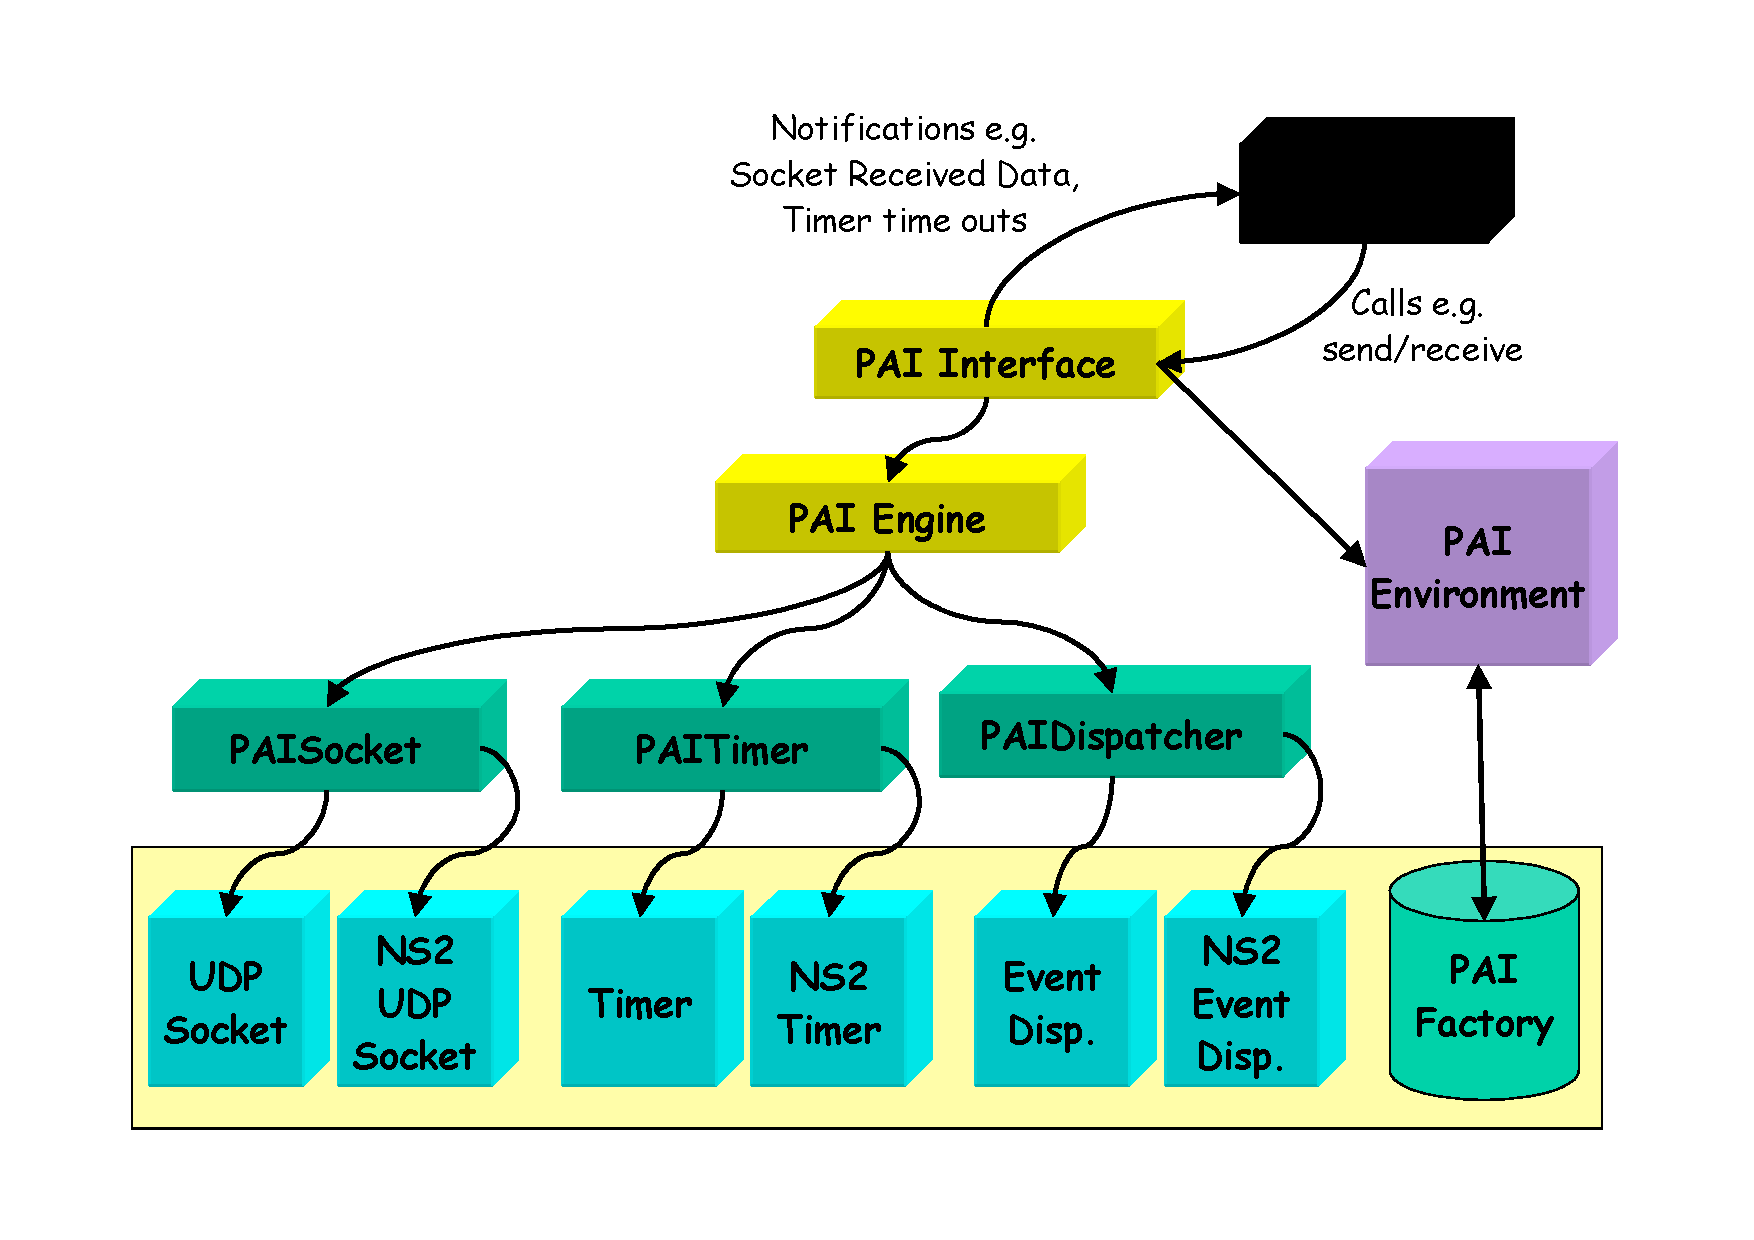
\includegraphics[scale=0.4]{images/paiFactory}
\caption{The PAI interface uses the Factory design pattern to create
a common high level interface to whatever sockets or underlying timers
the programmer is using.} 
\label{pai:fig:factory}
\end{figure}


\section{Programming PAI}



\begin{figure}
\centering
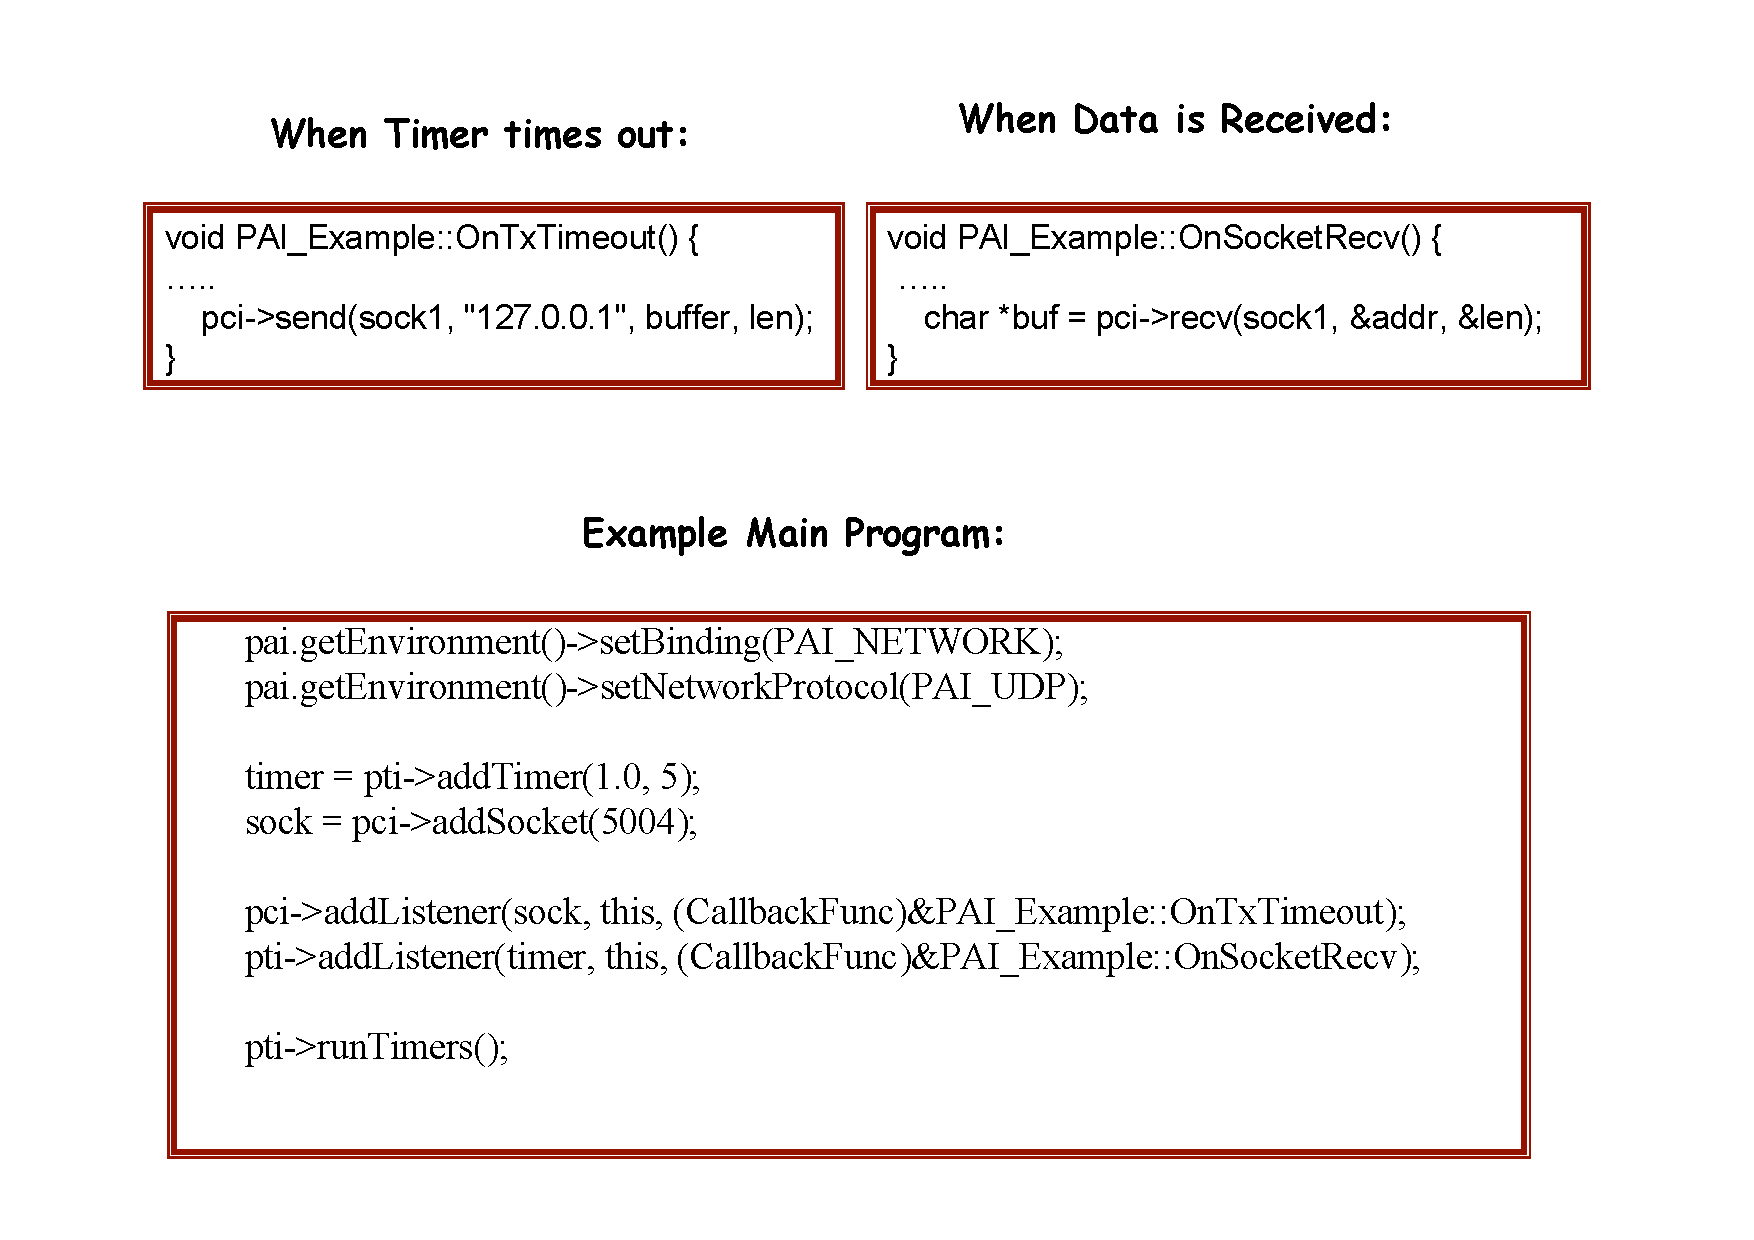
\includegraphics[scale=0.4]{images/paiExample}
\caption{An PAI code example, showing how you would implemented the 
standard Protolib demonstration, which sets of a 1 second timer and sends
data between two nodes.} 
\label{pai:fig:example}
\end{figure}


\section{Using PAI within NS2: The C++ Side}
\label{jni:nodeint}

\index{NS2}

The Java PAI interface described in the last Chapter can be used 
directly by C++ applications within NS2.  This chapters discusses
the C++ agent classes that have been written for \agentj and
how these can be used with PAI to pass data between NB2 nodes
and to set off timers.

\section{Ns2 Agents}

There are typically two main components within an NS2 scenario:

\begin{enumerate}
\item \textbf{C++ Agent:} This is used to represent the C++ behaviour
within Ns2.  Examples of agents could include transport protocols e.g.
UDP agent, TCP agent etc.  Agents can also be use to implement 
applications (using Protolib) or to broker them. 
\item \textbf{TCL Script:} This sepcifies which NS2 C++ agents will be used
and also to paint the scenario of the simulation you wish to perform
within the simulation environment.
\end{enumerate}

\begin{figure}
\centering
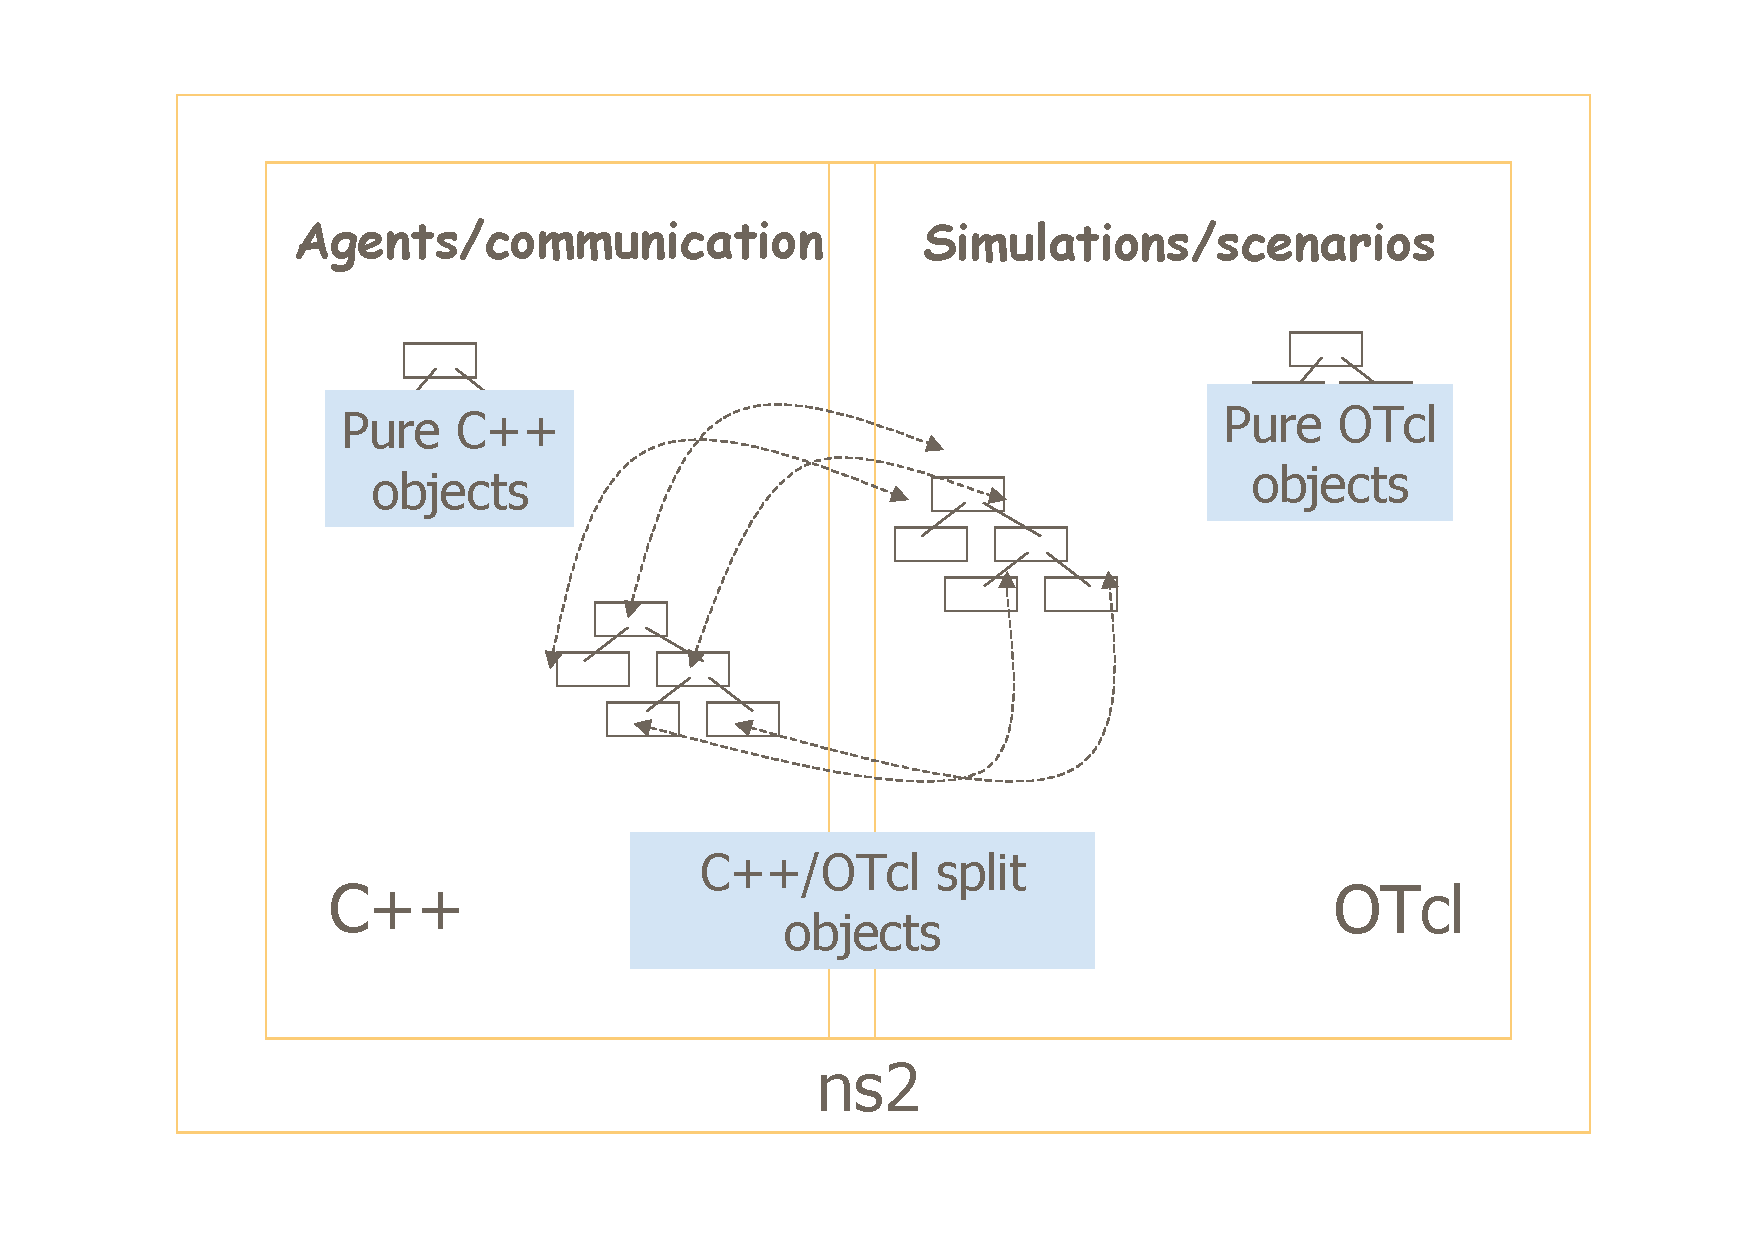
\includegraphics[scale=0.4]{images/paiAgentsTCLandC}
\caption{An overview of how TCL interacts with C++ agents within Ns2 } 
\label{paiagent:fig:paiAgentsTCLandC}
\end{figure}

Figure \ref{paiagent:fig:paiAgentsTCLandC} illustrates how these two
components interacts within NS2.  The TCL script sets up the environment,
e.g., the communication links, the underlying network core, and specifies
which agents are going to be used  within the simulation. An example
script is given below, which simply creates a BasicAgent class and
invokes a 'hello' command on that agent.

\footnotesize
\begin{verbatim}
set ns_ [new Simulator]

# Create two nodes
set n1 [$ns_ node]
set n2 [$ns_ node]

# Put a link between them
$ns_ duplex-link $n1 $n2 64kb 100ms DropTail
$ns_ queue-limit $n1 $n2 100
$ns_ duplex-link-op $n1 $n2 queuePos 0.5
$ns_ duplex-link-op $n1 $n2 orient right

set p1 [new Agent/BasicAgent]
$ns_ attach-agent $n1 $p1

puts "Starting simulation ..."

$ns_ at 0.0 "$p2 hello"
$ns_ at 1.0 "finish $ns_"

proc finish {ns_} {
$ns_ halt
delete $ns_
}

$ns_ run
\end{verbatim}
\normalsize

As you can see from the script, two Ns2 nodes are created and
a network link is specified between them. We then create
a custom Agent (called Basic Agent) and invoke a simple command on
that agent.   We are interested here in how such commands get 
passed to the agents.  For specifics and a compendium of 
example scripts and agents can be found in the Ns-2 manual
at the web site \cite{ns2}.

TCL scripts communicate with the C++ agents that they create by
passing them commands.  These commands get passes to a
standardized method within the C++ Agent, called:

\footnotesize
\begin{verbatim}
int PAIAgent::command(int argc, const char*const* argv) {
\end{verbatim}
\normalsize

\noindent where, conventionally (as in main()), the arguments provide the following information:

\begin{itemize}
\item \textbf{argc:} specifies the number of strings representing the command
and arguments which are being sent (i.e. args 1 contains the command and 
2 onwards specifies the arguments for the command).    
\item \textbf{argv:} These contain the actual strings representing the command
and its arguments.
\end{itemize}

Therefore, a command, such as:

\footnotesize
\begin{verbatim}
$ns_ at 0.0 "$p2 hello"
\end{verbatim}
\normalsize

\noindent would be caught by the following command method implementation:


\footnotesize
\begin{verbatim}
int PAIAgent::command(int argc, const char*const* argv) {

    if (2 == argc) {
        if (!strcmp(argv[1], "hello")) {
		cout << "BasicAgent: received a hello! " << endl;
                return TCL_OK;			
                }
        // else if  ... 
        }

    // invoke the command from the next object up in the Agent class hierarchy
    
    return NsProtoAgent::command(argc, argv);
}	
\end{verbatim}
\normalsize

The PAI agents, described in the next section build upon this basic 
framework and Protolib to allow real applications to be run within the
NS2 simulation environment. 
  
\section{PAI Agents and Protolib}

\begin{figure}
\centering
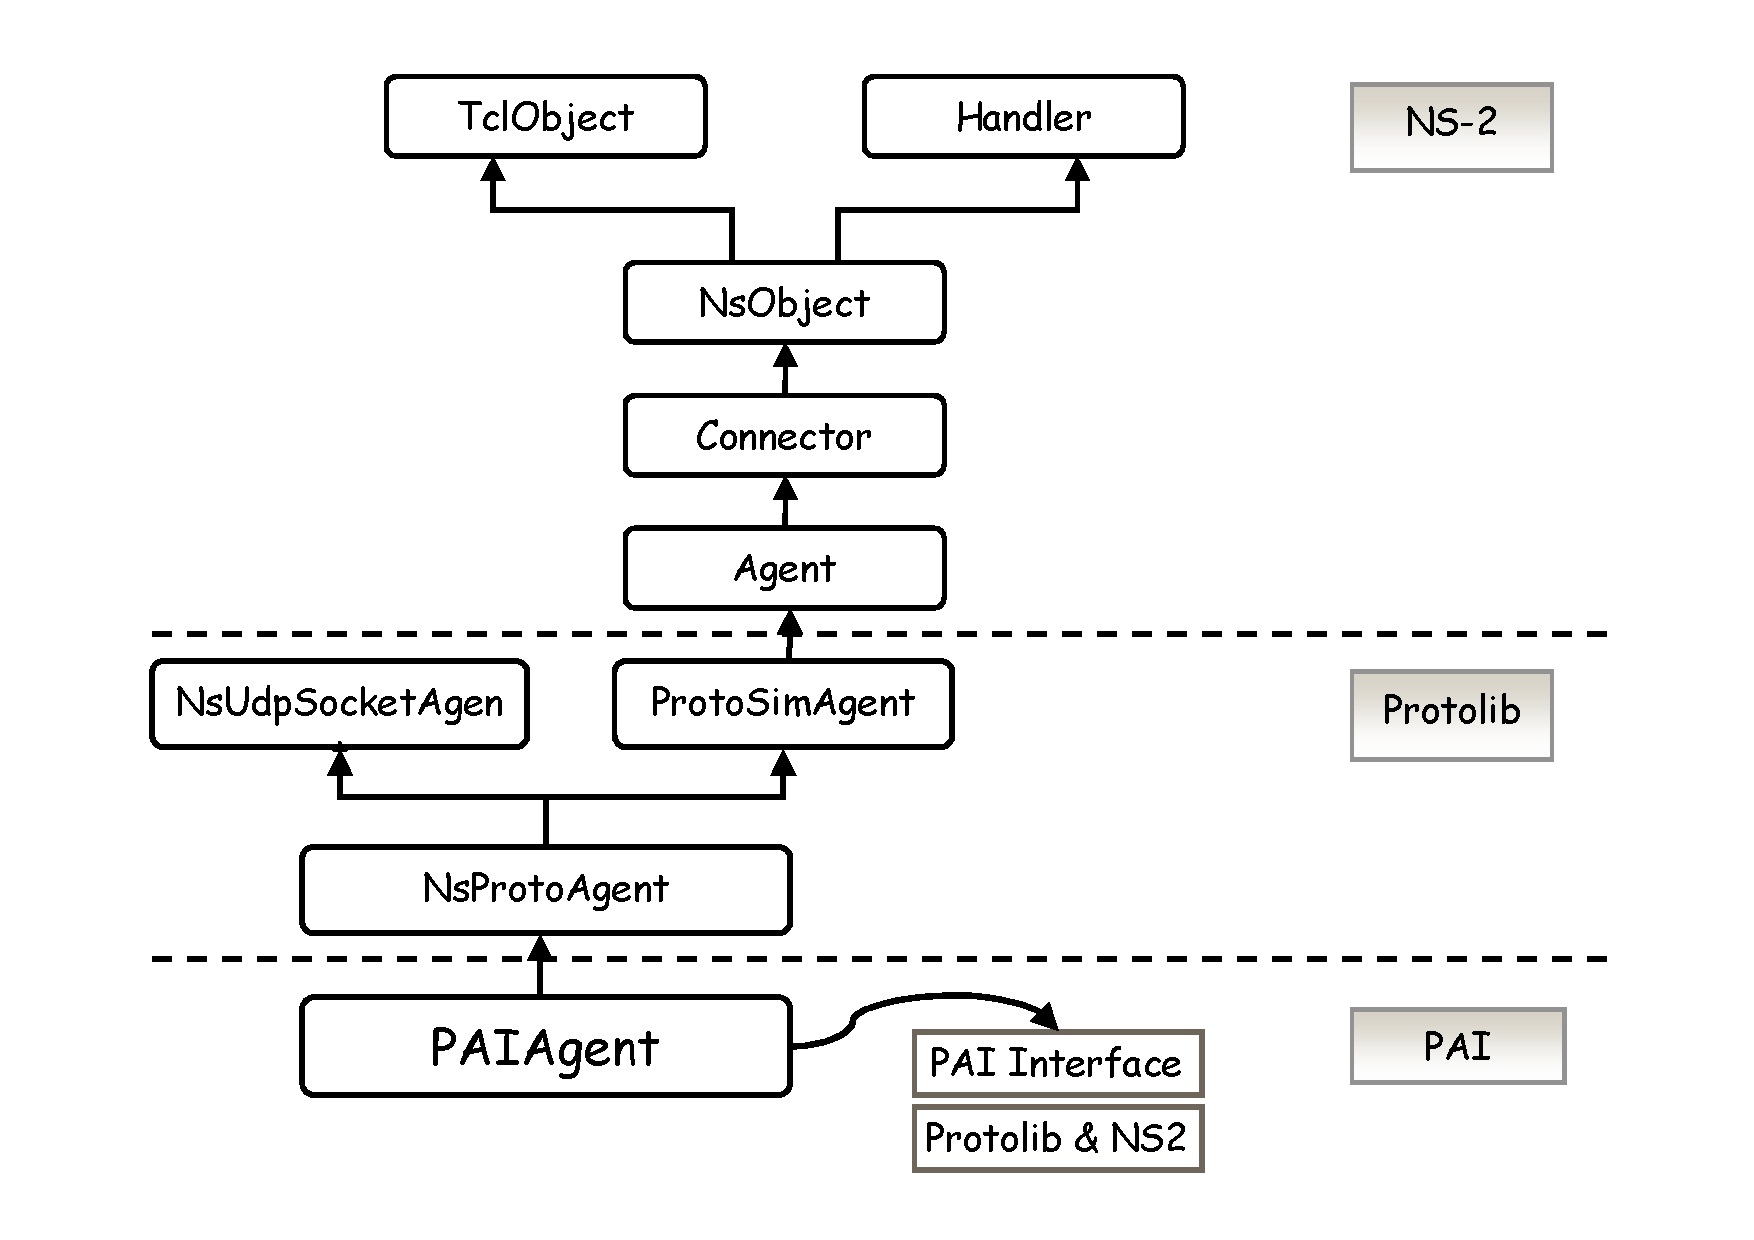
\includegraphics[scale=0.4]{images/paiAgentsClassHeirarch}
\caption{The Class structure of the NS2, Protolib and PAI classes to form the 
PAI agent hierarchy within NS2} 
\label{jni:fig:paiAgentsClassHeirarch}
\end{figure}

\section{Conclusion}

